%%%%%%%%%%%%%%%%%%%%%%%%%%%%%%%%%%%%%%%%%%%%%%%%%%%%%%%%%%%%%%%%%%%%%%
%
% Institut für Rechnergestuetzte Automation
% Forschungsgruppe Industrial Software
% Arbeitsgruppe ESSE
% https://security.inso.tuwien.ac.at/
% lva.security@inso.tuwien.ac.at
%
%%%%%%%%%%%%%%%%%%%%%%%%%%%%%%%%%%%%%%%%%%%%%%%%%%%%%%%%%%%%%%%%%%%%%%

\documentclass[12pt,a4paper,titlepage,oneside]{scrartcl}
\newcommand{\lang}{de}
\usepackage{esseProtocol}

%%%%%%%%%%%%%%%%%%%%%%%%%%%%%%%%%%%%%%%%%%%%%%%%%%%%%%%%%%%%%%%%%%%%%%
%
% FOR STUDENTS
%
%%%%%%%%%%%%%%%%%%%%%%%%%%%%%%%%%%%%%%%%%%%%%%%%%%%%%%%%%%%%%%%%%%%%%%

% Team number or "0" for Lab0
%TODO team number
\newcommand{\team}{48}
% Date
%TODO fill in creation date
\newcommand{\datum}{27.11.2018}
%TODO lab number
% valid values: "Lab0", "Lab1" (be sure to use Uppercase for first character)
\newcommand{\lab}{Lab1}

%TODO name of course
\newcommand{\lvaname}{Introduction to Security}
%TODO number of course
\newcommand{\lvanr}{183.594}
%TODO year and term, for example: "SS 2012", "WS 2012", "SS 2013", etc.
\newcommand{\semester}{WS 2018}

% Student data in Lab0 or 1. student of team in Lab1
\newcommand{\studentAName}{Tristan Ulreich}
\renewcommand{\studentAMatrnr}{01326158	}

% 2. student of team in Lab1, for Lab0 or if your team has less students, remove these 2 lines
\newcommand{\studentBName}{Jonathan Weber}
\renewcommand{\studentBMatrnr}{01525243}

% 3. student of team in Lab1, for Lab0 or if your team has less students, remove these 2 lines
\newcommand{\studentCName}{Otto Mustermann}
\renewcommand{\studentCMatrnr}{0815421}

% 4. student of team in Lab1, for Lab0 or if your team has less students, remove these 2 lines
\newcommand{\studentDName}{Otto Mustermann}
\renewcommand{\studentDMatrnr}{0995421}

% 5. student of team in Lab1, for Lab0 or if your team has less students, remove these 2 lines
\newcommand{\studentEName}{Otto Mustermann}
\renewcommand{\studentEMatrnr}{0236214}

%%%%%%%%%%%%%%%%%%%%%%%%%%%%%%%%%%%%%%%%%%%%%%%%%%%%%%%%%%%%%%%%%%%%%%
%
% DO NOT CHANGE THE FOLLOWING PART
%
%%%%%%%%%%%%%%%%%%%%%%%%%%%%%%%%%%%%%%%%%%%%%%%%%%%%%%%%%%%%%%%%%%%%%%

\newcommand{\colormode}{color}
\newcommand{\dokumenttyp}{Abgabedokument \lab}

\begin{document}

\maketitle
\setcounter{section}{0}
\setcounter{tocdepth}{2}
\tableofcontents

%%%%%%%%%%%%%%%%%%%%%%%%%%%%%%%%%%%%%%%%%%%%%%%%%%%%%%%%%%%%%%%%%%%%%%
%
% CONTENT OF DOCUMENT STARTS HERE
%
%%%%%%%%%%%%%%%%%%%%%%%%%%%%%%%%%%%%%%%%%%%%%%%%%%%%%%%%%%%%%%%%%%%%%%

\section{Ueberschrift 1}

\subsection{Hinweise}
\emph{Hinweise:}
\begin{itemize}
    \item Verwenden sie entweder diese deutsche Version oder die englische Version in \lstinline{protocol.tex}
    \item Setzen sie alle Variablen nach \emph{FOR STUDENTS} in der .tex Datei
    \item Ersetzen sie die Platzhalter für ihre Namen und MatNr.
    \item Löschen sie diese Sektion über Hinweise und die folgenden Beispiel-Kapitel
    \item Achten sie auf geforderte Formate und Anforderungen an die Dateinamen
    \item Führen Sie \lstinline{pdflatex} mindestens 2 mal aus, damit die Referenzen und Seitenzahlen richtig im PDF dargestellt werden
    \item Sie koenen dazu auch das Makefile verwenden: \lstinline{make de}
\end{itemize}

\subsection{Sub-Ueberschrift 1}
Lorem ipsum dolor sit amet, consetetur sadipscing elitr, sed diam nonumy eirmod tempor invidunt ut labore et dolore magna aliquyam erat, sed diam voluptua. At vero eos et accusam et justo duo dolores et ea rebum. Stet clita kasd gubergren, no sea takimata sanctus est Lorem ipsum dolor sit amet. Lorem ipsum dolor sit amet, consetetur sadipscing elitr, sed diam nonumy eirmod tempor invidunt ut labore et dolore magna aliquyam erat, sed diam voluptua. At vero eos et accusam et justo duo dolores et ea rebum. Stet clita kasd gubergren, no sea takimata sanctus est Lorem ipsum dolor sit amet.

\subsection{Sub-Ueberschrift 2}
Lorem ipsum dolor sit amet, consetetur sadipscing elitr, sed diam nonumy eirmod tempor invidunt ut labore et dolore magna aliquyam erat, sed diam voluptua. At vero eos et accusam et justo duo dolores et ea rebum. Stet clita kasd gubergren, no sea takimata sanctus est Lorem ipsum dolor sit amet. Lorem ipsum dolor sit amet, consetetur sadipscing elitr, sed diam nonumy eirmod tempor invidunt ut labore et dolore magna aliquyam erat, sed diam voluptua. At vero eos et accusam et justo duo dolores et ea rebum. Stet clita kasd gubergren, no sea takimata sanctus est Lorem ipsum dolor sit amet.

\section{Intranet}

\subsection{Netzwerk Dump}
Um den Netzwerkdump zu erstellen habe ich mich mittels ssh von meiner tese umgebung auf den Scan-Host verbunden welche in meinem Zeitslot im Tuwel bekanngegeben wurde. \\
\lstinline{ssh 10.10.15.101} \\
Mit dem folgendem Befehl aus der aircrack-ng suite habe ich die Wireless-Card in den Monitor Mode versetzt. Dieser Mode erlaubt es alle Wireless-Packets zu empfangen, auch jene die nicht für mich bestimmt waren.
\lstinline{airmon-ng start wlan} \\
Dieser Befehl erstellt ein weiteres Interface welches als suufix mon enthält \( wlanmon \). \\
Mittels dem Befehl \lstinline{airodump-ng wlanmon} startet die Aufzeichnung des Packetverkehrs. Solange dieser Befehl l\"auft wird aufgezeichnet. Weiters wird eine Tabelle mit den Access Points und den gerade aktiven Clients angezeigt. \\
Für eine Aufgabe ist es nötig authentification pakete aufzuzeichnen. Um dies zu erreichen habe ich mittels einer zweiter ssh Verbindung ident zu jener bereits beschriebenen folgenden Befehl ausgeführt. \\
\lstinline{aireplay-ng -0 10 -a 58:6D:8F:A9:25:53 -c [client MAC Address ] "wlanmon"} \\
Die erste Option gibt an wie viele Versuche unternommen werden sollen den Client zu deauthentifizieren. Die Option -a gibt die MAC Adresse des Access Points an und die Option -c die Client MAC Adresse, welche eine von den Adressen ist welche mit dem befehl \lstinline{airodump-ng wlanmon} angezeigt wurden. \\
Anschließend habe ich den erstellten Netzwerk Dump mittels ssh tunneling: \\
\lstinline{ tunel:ssh -L 9000:10.10.15.101:22 -p 12345 e01525243@tese.inso.tuwien.ac.at, sftp -oPort=9000 is_team48@localhost } \\
auf meinen Computer kopiert.


\subsection{Email}

Für diese Challenge habe ich das Netzwerkdumfile mit der Endung \lstinline{ .cap }  mit Wireshark geöffnet und nach SMTP paketen gefiltert. Eine Paket mit PlainText hat meine Aufmerksamkeit ergriffen und ich nutzte die Funktion von Wireshark den TCP Stream zu folgen. Daraufhin wurde mir jene Nachricht aus Abbildung 1 angezeigt aus welcher ich einfach das Passwort auslesen konnte.

%bild hier emailIntra
\begin{figure}[h!]
  \centering
  \fbox{
    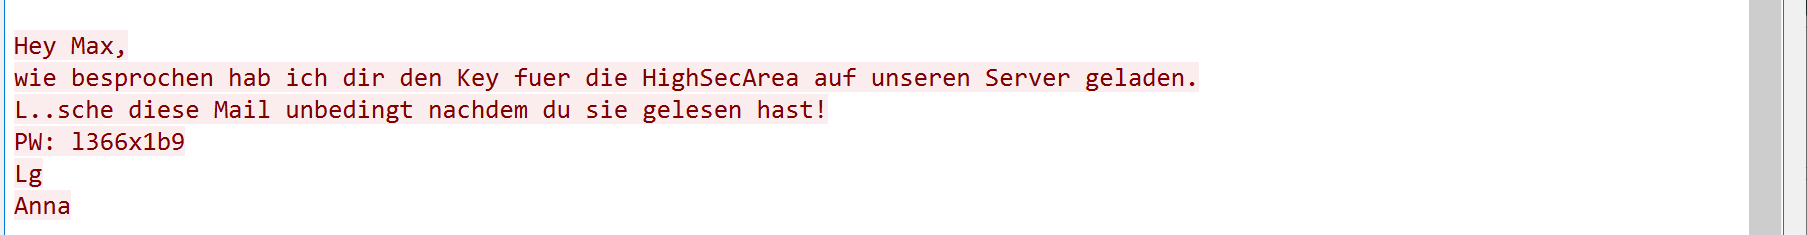
\includegraphics[width=0.8\textwidth]{./imgs/emailintranet.PNG}
  }
  \caption{SMTP Packet}
  \label{fig:Abilldung 1}
\end{figure}


\subsection{Voip}
Für diese CHallenge habe ich den Menüpunkt \lstinline{ Telephony } in Wireshark genutzt und dann über \lstinline{ Play Streams } abgespielt. Die Kontonummer könnte ich somit recht einfach heraushören. 


\subsection{IRC}
Um diese Challenge zu lösen habe ich in Wireshark den Filter \lstinline{irc } benutzt und dann die Option \lstinline{ Follow TCP STream }. Es wird mir ein chat verlauf angezeigt aus dem ich den Hash der Files auslesen kann. Zu sehen in Abbildung 2.

\begin{figure}[h!]
  \centering
  \fbox{
    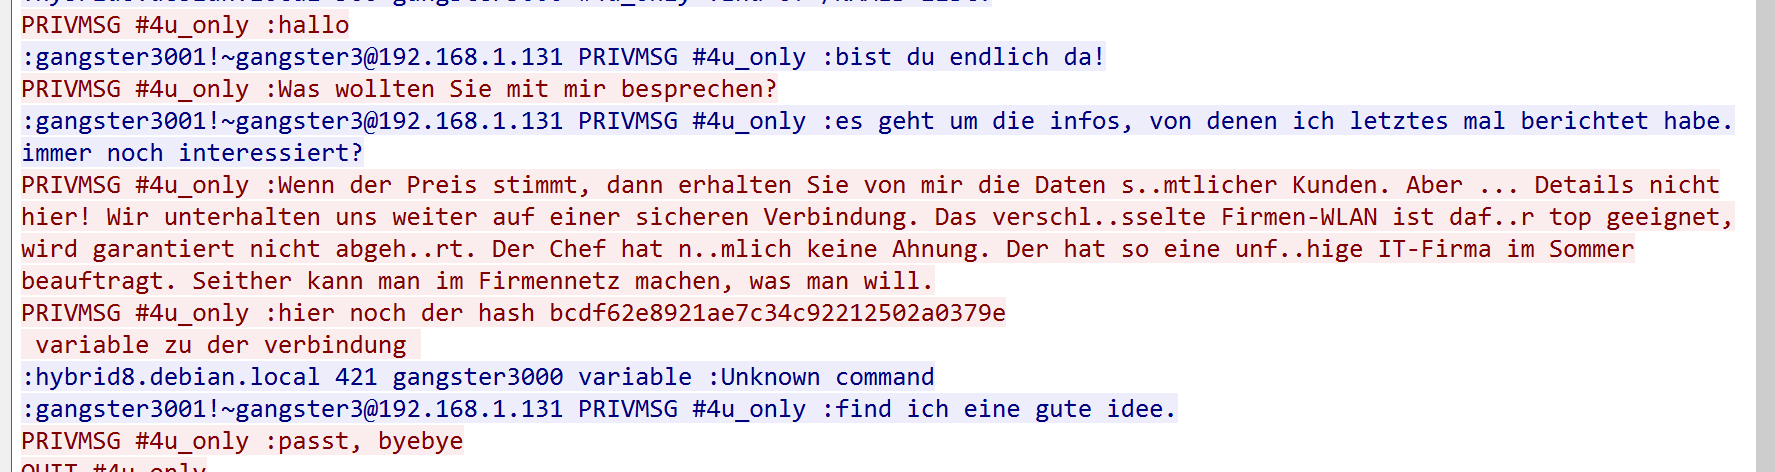
\includegraphics[width=0.8\textwidth]{./imgs/ircintra.PNG}
  }
  \caption{irc chat}
  \label{fig:Abilldung 2}
\end{figure}



\subsection{Wlan-Passwort}
Um die verschlüsselte Kommunikation in Netzwerk SecureHotdog sehen zu können musste für diese Challenge das Wlan Passwort mittels einer Worldlist erraten werden. Ich habe eine deutsche Wordlist verwendet und das Passwort mit Hilfe der aircrack Suite erraten. Folgender Befehl wurde angewandt. \\
\lstinline{ aircrack-ng dumpfile_20181125_200520-01.cap -w  ../worklists/german.dic } \\
Als korrektes Passwort ist bei dieser Methode Gitarrenspiel angezeigt worden. Mit Hilfe dessen ich nun den Netzwerk Dump entschlüsseln konnte. \\
\lstinline{airdecap-ng -e SecureHotDog -p Gitarrenspiel dumpfile_20181125_200520-01.cap  } 



\subsection{FTP}
Bei dieser Challenge musste der Name und Passwort des FTP Servers herausgefunden werden. Dies ist sehr leicht zu schaffen indem als Filter in Wireshark im entschlüsselten Netzwerk Dump ( siehe 2.5 ) \lstinline{ ftp } verwendet wird. Zu sehen in Abbildung 3.

\begin{figure}[h!]
  \centering
  \fbox{
    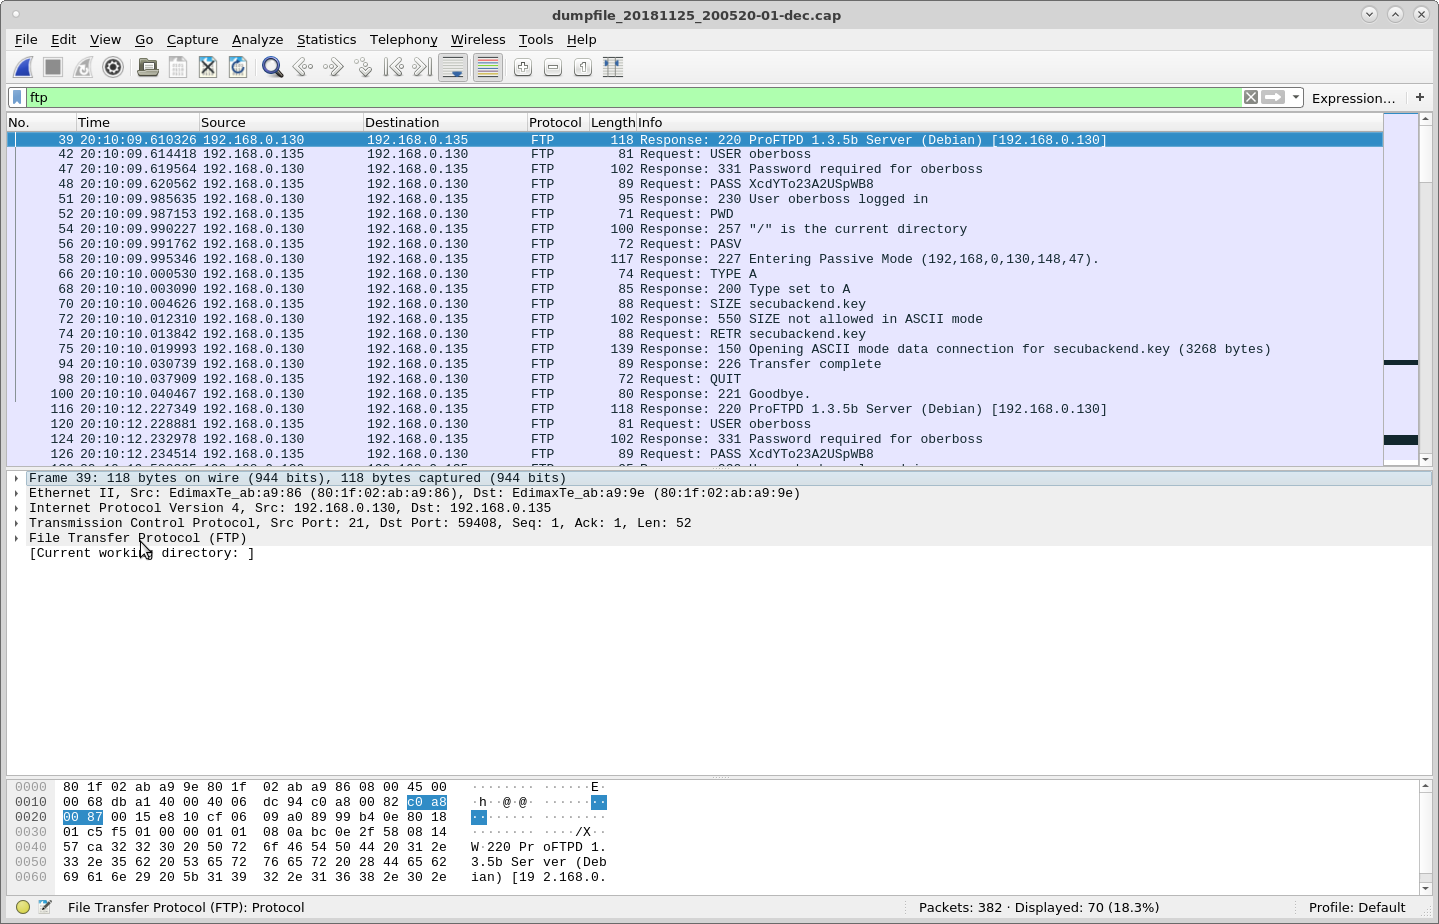
\includegraphics[width=0.8\textwidth]{./imgs/ftpintra.PNG}
  }
  \caption{ftp pakete}
  \label{fig:Abilldung 3}
\end{figure}

\subsection{FTP 2}
Um den Namen des Files herauszufinden, habe ich zuerst im entschlüsselden Netzwerk Dump (siehe 2.5) als Filter \lstinline{ ftp-data } verwendet. Hier habe ich erfahren, dass ein private key versendet wurde. Mit dem Filter \lstinline{ ftp } habe ich nun gesehen das ein File namens secubackend.key angefordert wurde.

\subsection{HTTPS}
Um das Logfile ansehen zu können habe ich in Wireshark im Netzwerk Dump des Netzwerkes HotDog den key aus aufgabe FTP 2 ( siehe 2.7 ) benutzt und unter Edit -> preferences -> SSL eingegeben um den SSL verkehr zu entschlüsseln. Zu sehen in Abblidung 4. 

\begin{figure}[h!]
  \centering
  \fbox{
    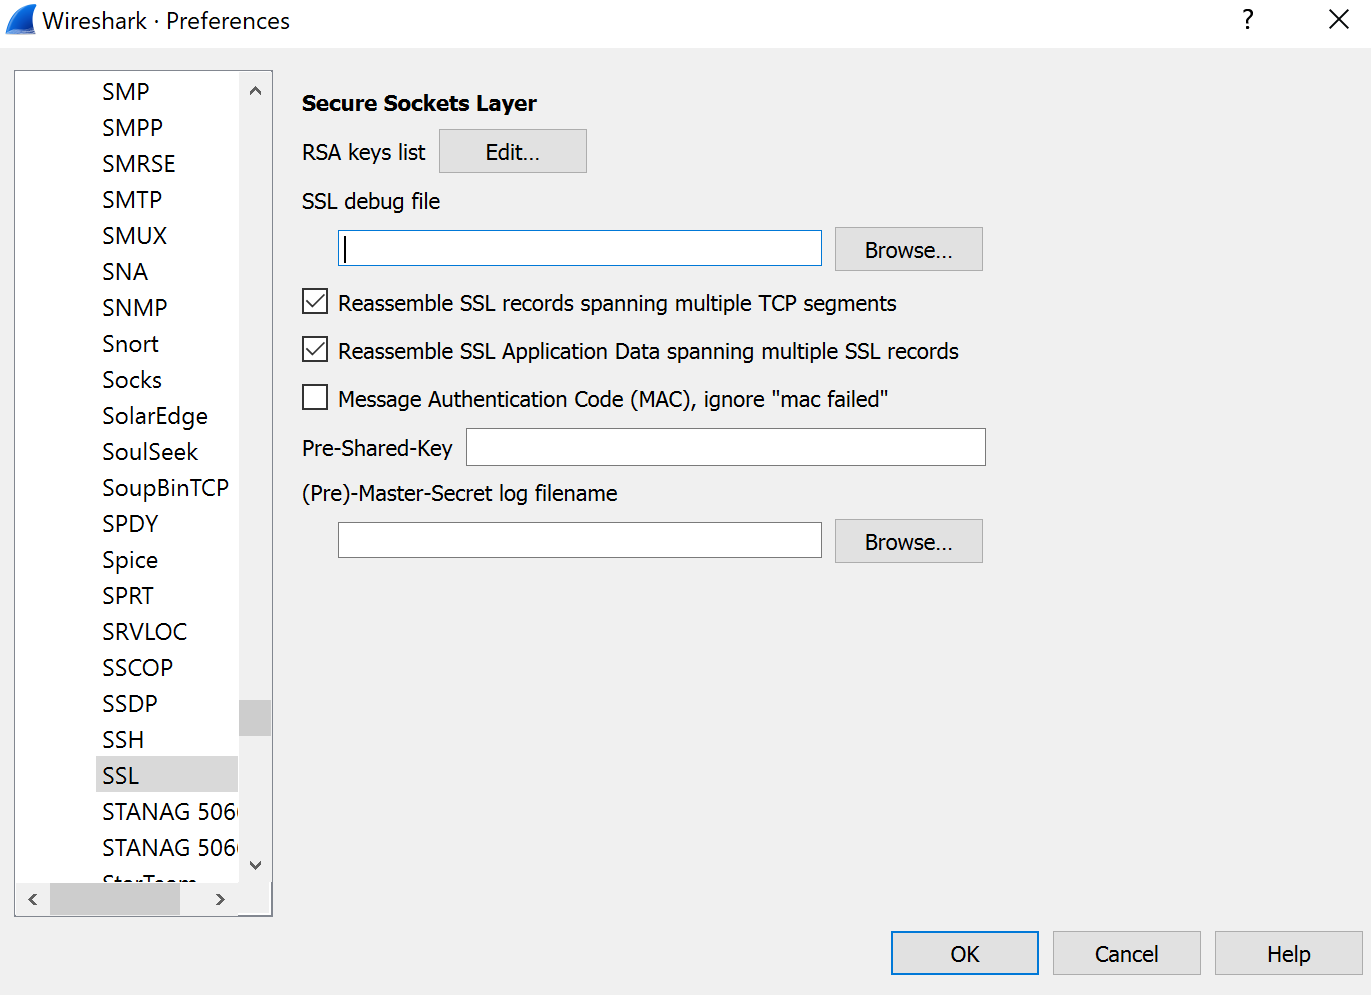
\includegraphics[width=0.8\textwidth]{./imgs/httpsintra1.PNG}
  }
  \caption{ftp pakete}
  \label{fig:Abilldung 4}
\end{figure}

\pagebreak

Nun konnte ich mit dem Filter ssl in Wireshark das http packet \lstinline{ GET /RXD7t1UFDS.log HTTP/1.1 } sehen. Mit der Option Follow ssl Stream habe ich das Logfile in Abbildung 5 einsehen können, aus welcher ich die gefragte Information auslesen konnte.

\begin{figure}[h!]
  \centering
  \fbox{
    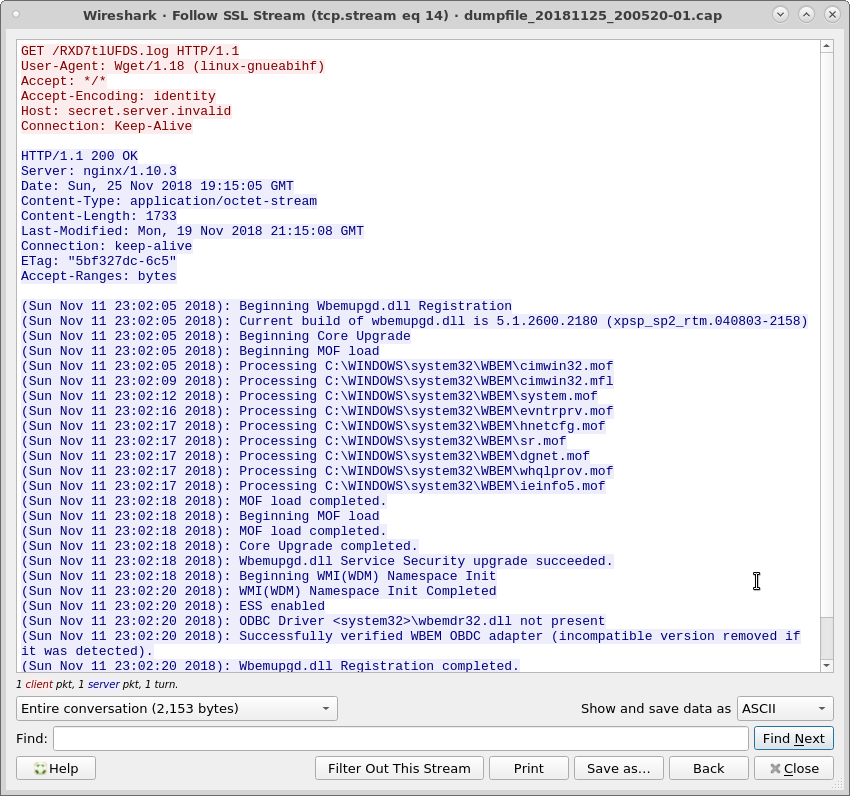
\includegraphics[width=0.8\textwidth]{./imgs/ssl1.PNG}
  }
  \caption{ftp pakete}
  \label{fig:Abilldung 5}
\end{figure}


\section{Scriptkiddie 101}

\subsection{Komprimierte Sicherheit }
Um die vierstellige Zahl zu finden habe ich mit \lstinline{ crunch 4 4 0123456789 } (min max erlaubte ziffern) ein File erstellt welches die zahlen 0000 bis 9999 beinhaltet und dann mittels meinem Script getPin.sh in Listing 1 ausgelesen. Wurde der richtige Code gefunden wird dieser ausgegeben.

\begin{lstlisting}[caption=getPin.sh,label=code:getPin.sh,style=simple]
#!/bin/bash 

while read password; do
    echo $password
    7z l ./open_me_easy.7z  * -p$password &> /dev/null 
    if [ $? -ne 2 ]
    then
       break
    fi       
done < ./pins.lst
\end{lstlisting}

\subsection{Proof of Work}
Um für diese Challenge die passende Ganzzahl zu finden, habe ich ein Perl Script \lstinline{ pfw.pl } geschrieben welches alle Zahlen ab 100 000 bis 200 000 durchprobiert und erkennt wenn genügend Nullen im Hash vorrangestellt sind. Zu sehen in Listing 2.

\begin{lstlisting}[caption=pfw.pl,label=code:pfw.pl,style=simple]
#!/bin/perl
#
use Digest::SHA;
use Digest::SHA qw(sha384_hex);
#
#my $suffix="o4ZdIddP3m0dAKNraZcTZQdoLAJCc9c6";  example
my $suffix="nTRr6tVWlIhn2wvSSAP55apk0IvqhHjb";

my $count = 100000;
my $content;
my $digest_h;
my $digest_b;
my $pos;

until ($count > 200000) {
  $content=$count . $suffix;	
  $digest_h = sha384_hex($content);
  $digest_b = hex2bin($digest_h);
  $pos = index($digest_b, '1');
  last if ($pos >= 17);
  $count++;
}  

print "data:       $content\n";
print "digest hex: $digest_h\n";
print "number:     $count\n";
print "digest bin: $digest_b\n"; 
print "leading 0:  $pos\n";

sub hex2bin {
        my $h = shift;
        my $hlen = length($h);
        my $blen = $hlen * 4;
        return unpack("B$blen", pack("H$hlen", $h));
}
\end{lstlisting}
 



\section{Forensik}

\subsection{Lizenzvertrag}
Um diese Aufgabe bearbeiten zu können, muss man zuerst das PDF erlangen.
Dazu habe ich mir die Datei in ~/ssh/config angelegt mit folgenden Daten:
\newline
\newline
Host lab \newline
HostName tese.inso.tuwien.ac.at \newline
Port 12345 \newline
User e01326158
\newline
\newline
Anschließend habe ich im Terminal den Befehl ssh -L 8048:10.10.10.100:8048 lab ausgeführt und somit eine SSH-Portweiterleitung instanziert.
Um nun das PDF herunterzuladen habe ich im Browser

$localhost:8048/downloads/Vertragsunterlagen_vertraulich.pdf$
\newline
\newline
eingegeben um das PDF herunterzuladen. Im Anschluss habe ich einfach den ausgeschwärzten Text im PDF markiert und somit die "geschwärzte" Zahl herausfinden können.

$1.804.167.212$


\subsection{Lizenz-Nachzahlung}
Um die Lizennachzahlung heruaszufinden, habe ich auf den ausgegrauten Text herangezoomt und festgestellt, dass die ursprüngliche Zahl noch leicht sichtbar ist. Ich hätte auch den Kontrast des PDF-Ausschnittes ändern können um den Preis sichtbarer zu machen.

$7.716.465.296$

\subsection{Crypto-Ref-ID}
Die Crypto-Ref-ID steht in den Eigenschaften des PDF Dokumentes.

$A13m7X07$

\subsection{Lizenz Berechtigung}
Die Zahlungsreferenz ist abseits des sichtbaren (für den PDF-Reader) PDFs gespeichert.

$RE151-774-T-31$


\subsection{Appendix 07}
Ich habe das PDF in LibreOffice-Draw geöffnet (PDF-Editor).
Hinter dem Bild ist ein zweites wesentlich kleineres Bild gespeichert, mit der Zeit.

$08:58:87$


\section{Manager9000}

\subsection{Schwachstelle finden}
Die Seite ist SQL Injection gefährdet. Mit dem Eingabedaten $' OR '1'='1' --$ in Nickname und Passwort kann fälschlicherweise eingeloggt werden.

\subsection{Wer schürft am meisten?}
Mittels $' OR '1'='1' );  drop table id$  kann die gesamte Liste der Miner ausgegeben werden, da bei Syntaxfehlern der ausgeführte SQL-Code ausgegeben wird, kann hier einfach die Eingabe angepasst werden. Nun muss nur noch der/die stärkste/er herausgesucht werden.

\subsection{Mein Wallet}

SELECT id, name, phone, country, city, street, number FROM contacts WHERE (name LIKE '\%
'OR '1'='1' ); SELECT id, name, phone, country, city, street, number FROM contacts ORDER BY name ;
('
\%' )

\section{Beispiele}

\subsection{Source Code formatieren}
Es folgen einige Beispiele wie Sourcecode in diesem Dokument formatiert und referenziert werden kann
(\hyperref[code:beispiel1]{siehe Listing~\ref*{code:beispiel1} auf Seite~\pageref*{code:beispiel1}} und \hyperref[code:beispiel2]{siehe Listing~\ref*{code:beispiel2} auf Seite~\pageref*{code:beispiel2}}).

Ebenso können kurzer Code oder kurze Befehle direkt in der Zeile in einem \lstinline{lstinline Block} mit typengleicher Schrift formatiert werden.

\lstinputlisting[caption=Example C/C++ file,label=code:beispiel1,style=c]{example.c}

\begin{lstlisting}[caption=Example bash script,label=code:beispiel2,style=simple]
#!/bin/bash
echo "Bash version ${BASH_VERSION}..."
for i in {0..10..2}
  do
     echo "Welcome $i times"
 done

echo "some very very very very very very very very very very very very very very very very very very very very long string"

exit 0;
\end{lstlisting}

\subsection{Bilder}

Es folgen einige Beispiele wie Bilder in diesem Dokument eingefuegt werden koennen
(\hyperref[fig:logo1]{siehe Abbildung~\ref*{fig:logo1} auf Seite~\pageref*{fig:logo1}}).

\begin{figure}[h!]
  \centering
  \fbox{
    
\includegraphics[width=0.4\textwidth]{./imgs/logos/esse-logo-color.png}
  }
  \caption{ESSE Logo}
  \label{fig:logo1}
\end{figure}


%%%%%%%%%%%%%%%%%%%%%%%%%%%%%%%%%%%%%%%%%%%%%%%%%%%%%%%%%%%%%%%%%%%%%%
%
% DO NOT CHANGE THE FOLLOWING PART
%
%%%%%%%%%%%%%%%%%%%%%%%%%%%%%%%%%%%%%%%%%%%%%%%%%%%%%%%%%%%%%%%%%%%%%%

\end{document}


